\svnid{$Id: section_ribbons.tex 1 2015-08-30 15:39:28Z mooiman $}

%-------------------------------------------------------------------------------
\section{Ribbons and toolbars}
\label{sec:ribbons}
The user can access the toolbars arranged in \menu{ribbons}. Failure mechanisms plug-ins can have their own specific \menu{ribbon}. The \menu{ribbon} may be auto collapsed by activating the \button{Collapse the Ribbon} button when right-mouse-clicking on the \menu{ribbon}.

%-------------------------------------------------------------------------------
\subsection{Ribbons (hot keys)}\label{subsec:gettingstarted_ribons}

WTI Ringtoets makes use of ribbons, just like Microsoft Office. You can use these ribbons for most of the operations. 
With the ribbons comes hot key functionality, providing shortcuts to perform operations.
If you press ``ALT'', you will see the letters and numbers to access the ribbons and the ribbon contents (i.e.\ operations). For example, ``ALT'' + ``H'' will lead you to the ``Home''-ribbon (\Fref{fig:ribbonhotkey}).

\textbf{\Note Implementation of the hot key functionality is still work in progress.}

\begin{figure}[H]
	\centering
	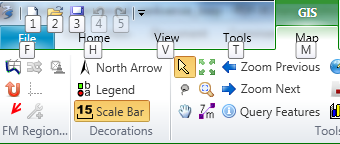
\includegraphics{Figures/Chapter_overview/ds_ribbon_hotkey.png}
	\caption{Perform operations using the hot keys} \label{fig:ribbonhotkey}
\end{figure}

%-------------------------------------------------------------------------------
\subsection{File}
\label{subsec:file}
The left-most \menu{ribbon} is the \menu{File} ribbon. It has menu-items comparable to most Microsoft applications. Furthermore, it offers users import and export functionality, as well as the \menu{Help} and \menu{Options} dialogs, as shown in \Fref{fig:ribbonfile} and \Fref{fig:dsoptions}.
%
\begin{figure} [H]
	\centering
		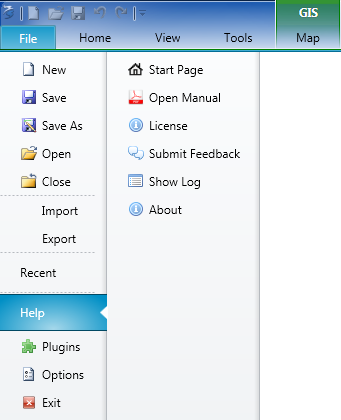
\includegraphics[width=0.6\textwidth]{Figures/Chapter_overview/ribbon_file.png}
	\caption{The \menu{File} ribbon.}
	\label{fig:ribbonfile}
\end{figure}
%
\begin{figure} [H]
	\centering
		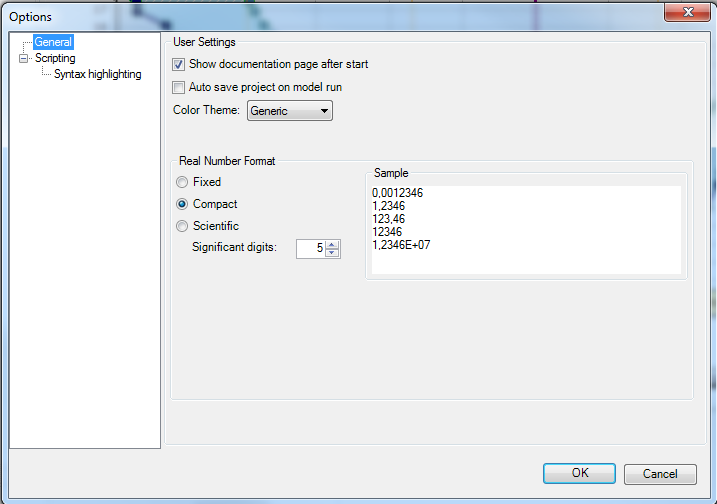
\includegraphics[width=\textwidth]{Figures/Chapter_overview/ds_options.png}
	\caption{The options dialog.}
	\label{fig:dsoptions}
\end{figure}

%-------------------------------------------------------------------------------
\subsection{Home}
\label{ssec:ribbonhome}
The second \menu{ribbon} is the \menu{Home} ribbon (\Fref{fig:ribbonhome}). It harbours some general features for clipboard actions, addition of items, running models, finding items within projects or views, and help functionality.
\begin{figure}[H]
	\centering
	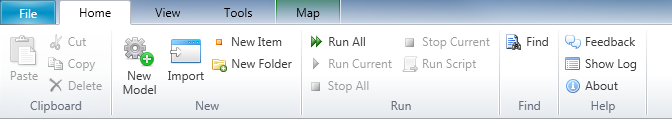
\includegraphics[width=1.0\textwidth]{Figures/Chapter_overview/ribbon_home.png}
	\caption{The \menu{Home} ribbon.}
	\label{fig:ribbonhome}
\end{figure}
%
%-------------------------------------------------------------------------------
\subsection{View}
\label{ssec:ribbonview}
The third \menu{ribbon} is the \menu{View} ribbon (\Fref{fig:ribbonview}). Here, the user can show or hide windows.
\begin{figure}[H]
	\centering
	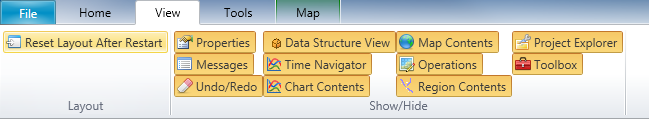
\includegraphics[width=0.5\textwidth]{Figures/Chapter_overview/ribbon_view.png}
	\caption{The \menu{View} ribbon.}
	\label{fig:ribbonview}
\end{figure}
%
%-------------------------------------------------------------------------------
\subsection{Tools}
\label{ssec:ribbontools}
The fourth \menu{ribbon} is the \menu{Tools} ribbon (\Fref{fig:ribbontools}). By default, it contains only the \menu{Open Case Analysis View} tool. Some model plug-ins offer the installation of extra tools that may be installed. These are documented within the user documentation of those model plug-ins. 
\begin{figure}[H]
	\centering
	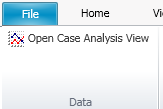
\includegraphics[width=0.2\textwidth]{Figures/Chapter_overview/ribbon_tools.png}
	\caption{The \menu{Tools} ribbon.}
	\label{fig:ribbontools}
\end{figure}
%
%-------------------------------------------------------------------------------
\subsection{Map}
\label{ssec:ribbonmap}
The last \menu{ribbon} is the \menu{Map} ribbon (\Fref{fig:ribbonmap}).
\begin{figure}[H]
	\centering
	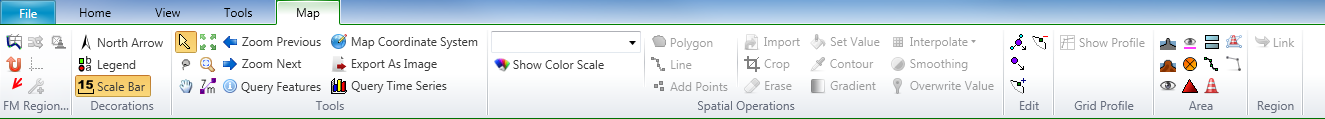
\includegraphics[width=1.0\textwidth]{Figures/Chapter_overview/ribbon_map.png}
	\caption{The \menu{Map} ribbon.}
	\label{fig:ribbonmap}
\end{figure}
%
This will be used heavily, while it harbours all \menu{Geospatial} functions, like:
\begin{itemize}
\item \menu{Decorations} for the map
\begin{itemize}
	\item North arrow
	\item Scale bar
	\item Legend
	\item ...
\end{itemize}
\item \menu{Tools} to customize the map view
\begin{itemize}
	\item Select a single item
	\item Select multiple items by drawing a curve
	\item Pan
	\item Zoom to Extents
	\item Zoom by drawing a rectangle
	\item Zoom to Measure distance
	\item ...
\end{itemize}
\item \menu{Edit} polygons, for example within a network, basin, or waterbody
\begin{itemize}
	\item Move geometry point(s)
	\item Add geometry point(s)
	\item Remove geometry point(s)
\end{itemize}
\item Creation of a model \menu{Network}, for example for \dflow
\begin{itemize}
	\item Add new Branch
	\item Split Branch
	\item Add Cross section
	\item Add Weir
	\item Add Pump
	\item ...
\end{itemize}
\end{itemize}
%
\Note The \menu{ribbons} adjust to the size of the application window. If, for what reason, the user wants to minimize the window, the ribbons might look like as shown in \Fref{fig:ribbonmapminimised}. Some of the \menu{ribbon} categories have been condensed into a single drop-down panel.
\begin{figure}[H]
	\centering
	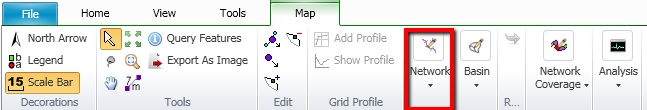
\includegraphics[width=0.8\textwidth]{Figures/Chapter_overview/ribbon_map_minimised.png}
	\caption{The ribbon with minimized categories.}
	\label{fig:ribbonmapminimised}		
\end{figure}
%
Still, all functions of the category can be activated as they will appear in the drop-down panel.
%
%-------------------------------------------------------------------------------
\subimport{chapters/}{ribbon_scripting}
%
%-------------------------------------------------------------------------------
\subsection{Quick access toolbar}
\label{ssec:Qaccestoolbar}
\Note The user can make frequently used functions available by a single mouse-click in the \menu{Quick Access Toolbar}, the top-most part of the application-window. Do this by right-mouse-clicking a ribbon item and selecting \menu{Add to Quick Access Toolbar}.
%
\begin{figure}[H]
	\centering
	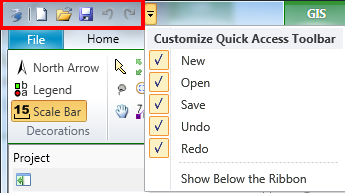
\includegraphics[width=0.6\textwidth]{Figures/Chapter_overview/quick_access_toolbar.png}
	\caption{The quick access toolbar.}
	\label{fig:qat}		
\end{figure}